\chapter{Demo}

A demo of our JavaScript implementation of Fortune's algorithm is available at \url{http://funbyjohn.com/voronoi/}. In general you can add points by clicking with the mouse, and if you click on a point while holding down shift you delete the point.
\[
    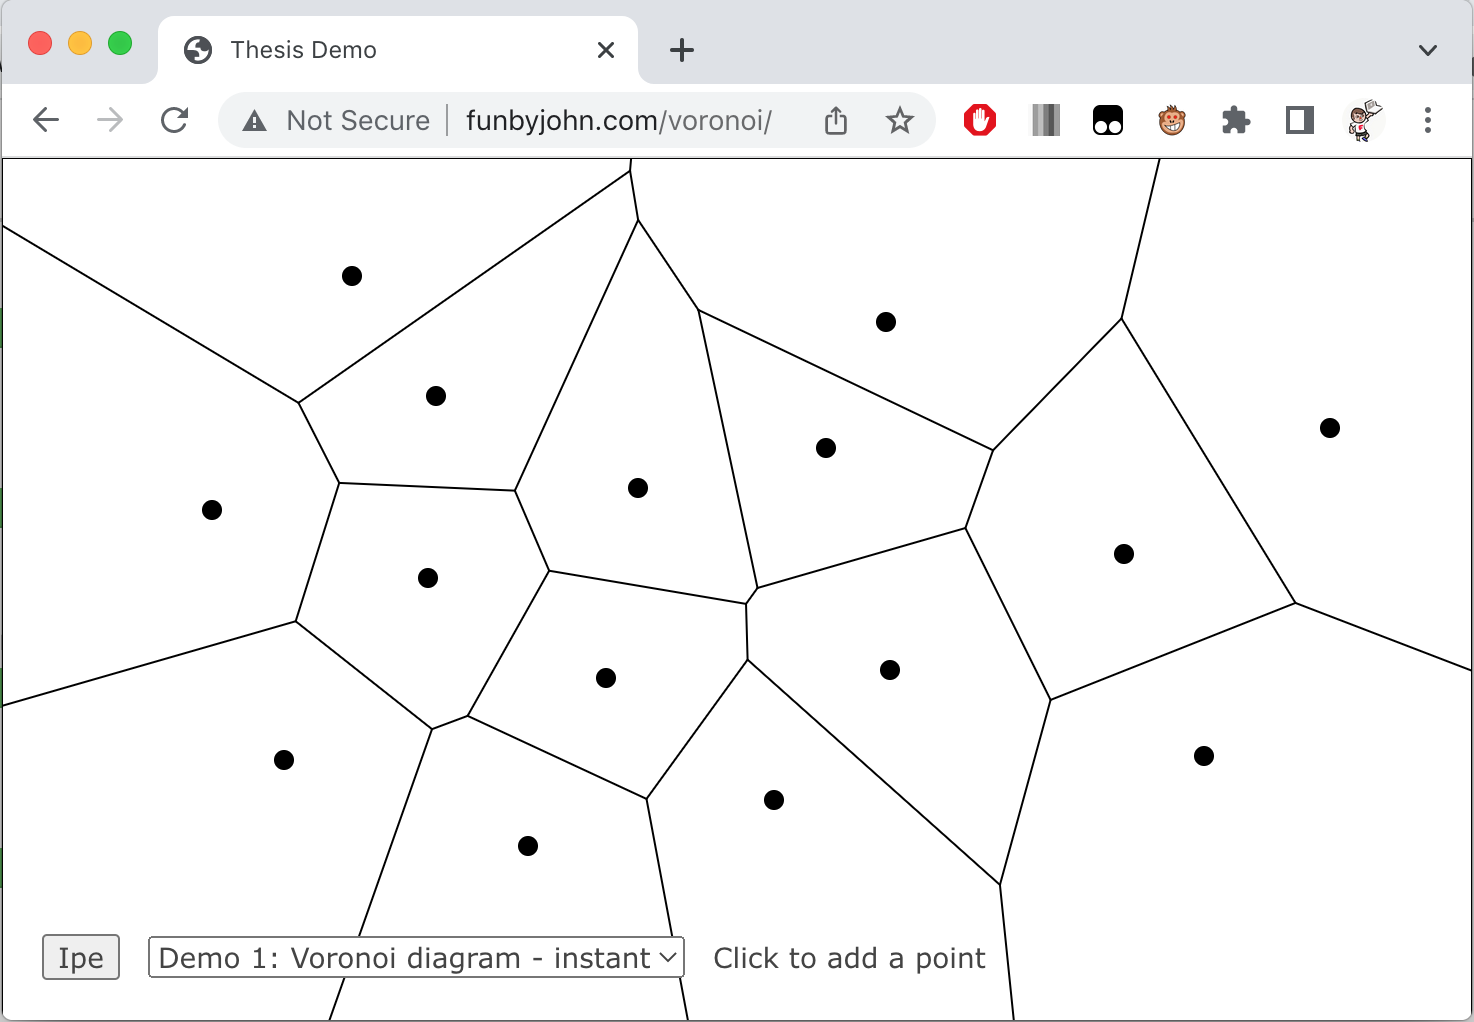
\includegraphics[width=\textwidth]{demo1}
\]
The first demo can be seen above. Here the Voronoi diagram is enclosed in a bounding box, and you may hide the bounding box by pressing the 6 key, and you can change its size by pressing the 7 and 8 keys.
\[
    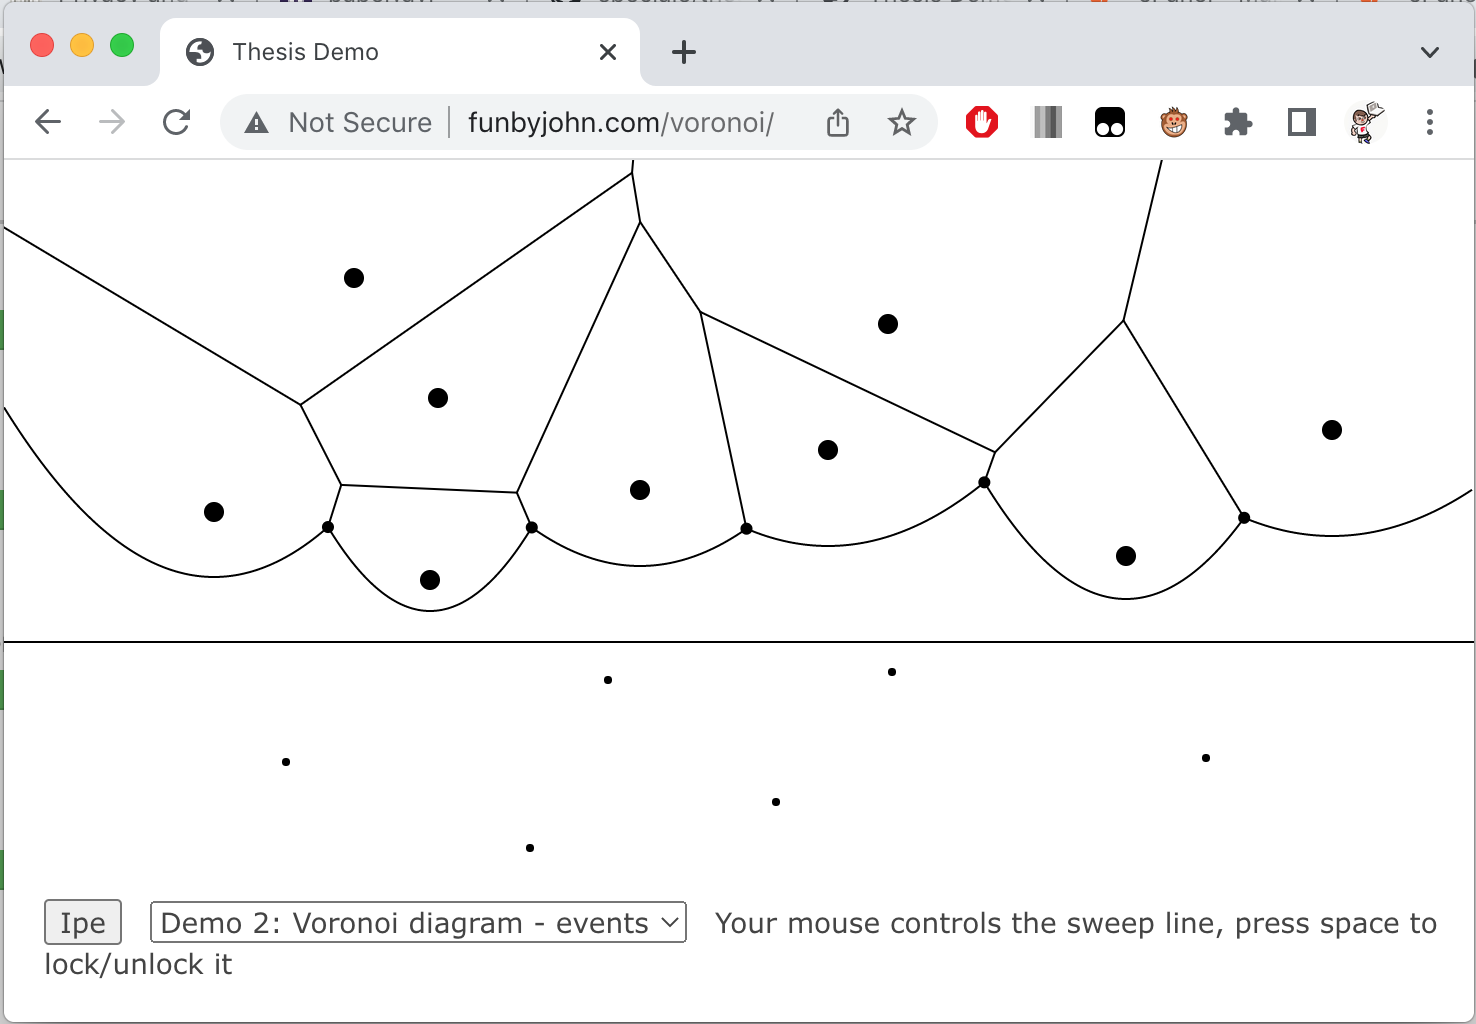
\includegraphics[width=\textwidth]{demo2}
\]
The second demo can be seen above. It shows the beach line, and you can move it up and down using the mouse. If you hold down shift the sweep line will move slower.
\[
    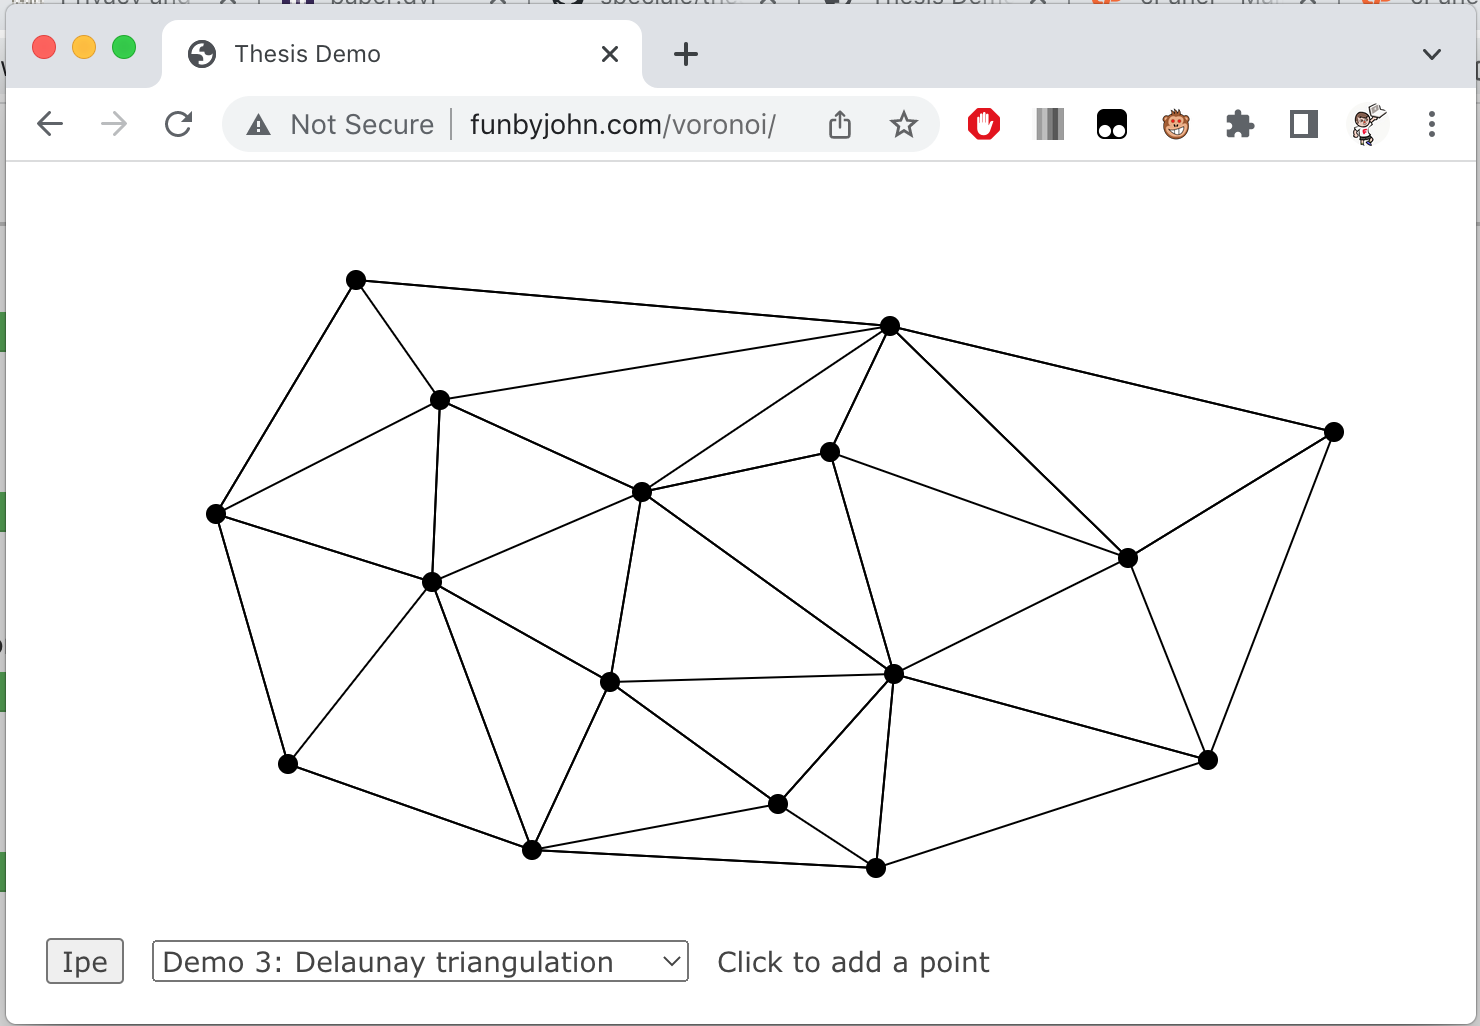
\includegraphics[width=\textwidth]{demo3}
\]
The final demo showcases the Delaunay triangulation, which is computed by taking the dual of the Voronoi graph.

\subsection*{Key legend}
Here is an overview displaying what every key does:
\begin{table}[H]
\centering
\begin{tabular}{ll}
\textbf{Key} & \textbf{Effect}                                           \\ \hline
1            & Toggle drawing the binary search tree in Demo 2           \\
2            & Toggle showing names of breakpoints in Demo 2             \\
3            & Toggle showing the oriented edges in the DCEL in Demo 2   \\
4            & Toggle showing face pointers in the DCEL in Demo 2        \\
5            & Toggle showing .next/.prev pointers in the DCEL in Demo 2 \\
6            & Toggle bounding box display in both Demo 1                \\
7            & Make bounding box smaller in Demo 1                       \\
8            & Make bounding box bigger in Demo 1                        \\
9            & Toggle showing circle events in Demo 2                    \\
Space        & Lock/unlock sweep line in Demo 2                          \\
Shift        & Hold down to make sweep line move slower in Demo 2        \\ \hline
\end{tabular}
\end{table}
Note that the face pointers and the .next/.prev pointers needs the oriented edges to be visible in order to work.

\subsection*{Warnings}
There are some bugs and numerical issues in the implementation at the time of writing. For a good time make sure to keep the following rules:
\begin{itemize}
    \item Make sure no points have the same $y$-value.
    \item Make sure that at most 3 points lie on the same circle.
    \item Don't place more than one point in the same spot.
\end{itemize}